\documentclass{article}
\usepackage[utf8]{inputenc}
\usepackage[italian]{babel}
\usepackage{amsfonts} 
\usepackage{graphicx}
\usepackage{amsmath} 
\usepackage{cancel}

\title{Exercises L2}
\author{Zanella Matteo}
\date{01 November 2023}

\begin{document}

\maketitle

\section*{2.1:}
\subsection*{2.1.1:}
Prove that $$S^2\leq\frac{1}{n-1}\sum_{i}(X_i-a)^2,\qquad\forall a\in\mathbb{R}$$
\newline
Since $S^2=\frac{1}{n-1}\sum_{i}(X_i-\overline{X})^2$, we can rewrite the inequality as follows:
\begin{align*}
    \cancel{\frac{1}{n-1}}\sum_{i}(X_i-\overline{X})^2&\leq\cancel{\frac{1}{n-1}}\sum_{i}(X_i-a)^2\\
    \sum_{i}(X_i-\overline{X})^2&\leq\sum_{i}(X_i-a)^2\\
    \sum_i(X_i^2-2X_i\overline{X}+\overline{X}^2)&\leq\sum_i(X_i^2-2X_ia+a^2)\\
    \cancel{\sum_iX_i^2}-2\overline{X}\sum_iX_i+\overline{X}^2\sum_i1&\leq\cancel{\sum_iX_i^2}-2a\sum_iX_i+a^2\sum_i1\\
    -2\overline{X}\sum_iX_i+n\overline{X}^2&\leq-2a\sum_iX_i+na^2\\
    2(\overline{X}-a)\sum_iX_i&\geq n(\overline{X}^2-a^2)\\
    2(\overline{X}-a)\frac{1}{n}\sum_iX_i&\geq\overline{X}^2-a^2\\
    2(\overline{X}-a)\overline{X}&\geq\overline{X}^2-a^2\\
    \overline{X}^2-2\overline{X}a+a^2&\geq0\\
    (\overline{X}-a)^2&\geq0\rightarrow \text{True}\,\,\forall a\in\mathbb{R}
\end{align*}
\subsection*{2.1.2:}
Prove that $$(n-1)\frac{S^2}{n}=\overline{X^2}-\overline{X}^2$$
\newline
\begin{align*}
    \frac{\cancel{n-1}}{n}\frac{1}{\cancel{n-1}}\sum_i(X_i-\overline{X})^2&=\frac{1}{n}\sum_iX_i^2-\overline{X}^2\\
    \cancel{\frac{1}{n}}\sum_i(X_i-\overline{X})^2&=\cancel{\frac{1}{n}}\sum_iX_i^2-n\overline{X}^2\\
    \cancel{\sum_iX_i^2}-2\overline{X}\sum_iX_i+\overline{X}^2&=\cancel{\sum_iX_i^2}-n\overline{X}^2\\
    -2n\overline{X}^2+n\overline{X}^2&=-n\overline{X}^2\\
    0&=0\rightarrow\text{True always}
\end{align*}
\section*{2.2:}
Given $X_1,...,X_n$ i.i.d. rv s.t. $X_i\sim F$
\subsection*{2.2.1:}
Prove that $$f_{X_{(1)}}(t)=n(1-F(t))^{n-1}f(t)$$($f_{X_{(1)}}(t)$ is the pdf of the minimum among the $X_i$)\\
\newline
$$P[X_i=t]=f(t)$$
$$P[X_i>t]=1-P[X_i<t]=1-F(t)$$
To find the pdf of the minimum, we have to compute the probability of $X_i$ being the smallest (say $t$), and all the other variabiles being greater than $t$ and sum it for each $X_i$:
$$f_{X_{(1)}}(t)=\sum_{i=1}^{n}\biggl[f_{X_i}(t)\prod_{j=1,j\neq i}^n(1-F_{X_j}(t))\biggr]$$
Since the variables are i.i.d., we can simplify the equation:
$$f_{X_{(1)}}(t)=\sum^nf(t)\prod^{n-1}(1-F(t))=nf(t)(1-F(t))^{n-1}$$
\subsection*{2.2.2:}
Prove that $$f_{X_{(n)}}(t)=n(F(t))^{n-1}f(t)$$($f_{X_{(n)}}(t)$ is the pdf of the maximum among the $X_i$)\\
\newline
With the same logic as before, we have to find the probability of $X_i$ being $t$ and all other variables being smaller than $t$ and sum it for each $X_i$:
$$f_{X_{(n)}}=\sum^nf(t)F(t)^{n-1}=nf(t)(F(t))^{n-1}$$
\subsection*{2.2.3:}
Since the variables are not independent anymore, we cannot simplify the formula seen before:
$$f_{X_{(1)}}(t)=\sum_{i=1}^{n}\biggl[P[X_i=t|X_k,\forall k\neq i]\prod_{j=1,j\neq i}^n(1-P[X_j<t|X_k,\forall k\neq j])\biggr]$$
$$f_{X_{(n)}}(t)=\sum_{i=1}^{n}\biggl[P[X_i=t|X_k,\forall k\neq i]\prod_{j=1,j\neq i}^n(P[X_j<t|X_k,\forall k\neq j])\biggr]$$
\subsection*{2.2.4:}
$$F_{X_{(3)}}(t)=4f(t)(F(t))^2(1-F(t))$$
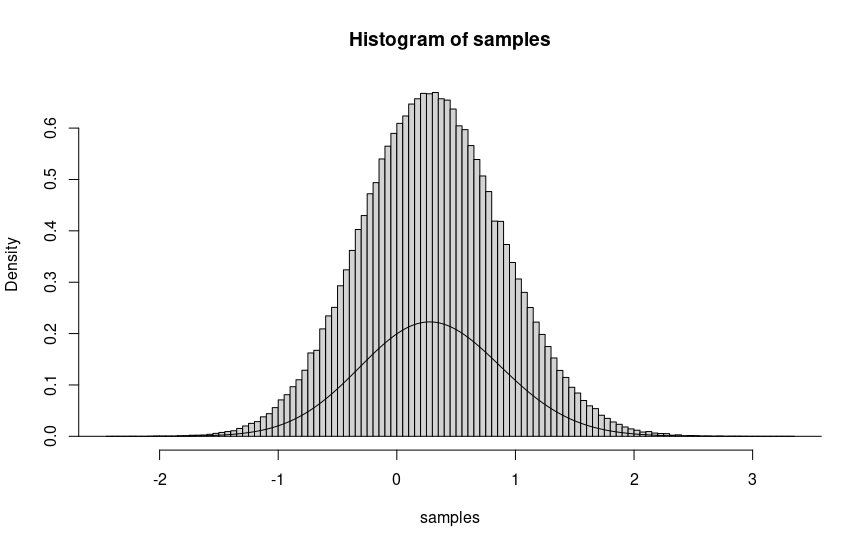
\includegraphics[width=\textwidth]{img/2-2-4.png}
\section*{2.3:}
For the observed sample:
$$8.935,\,0.492,\,6.951,\,4.102,\,0.111,\,2.699,\,3.255,\,6.254,\,2.120,\,29.389$$
\subsection*{2.3.1:}
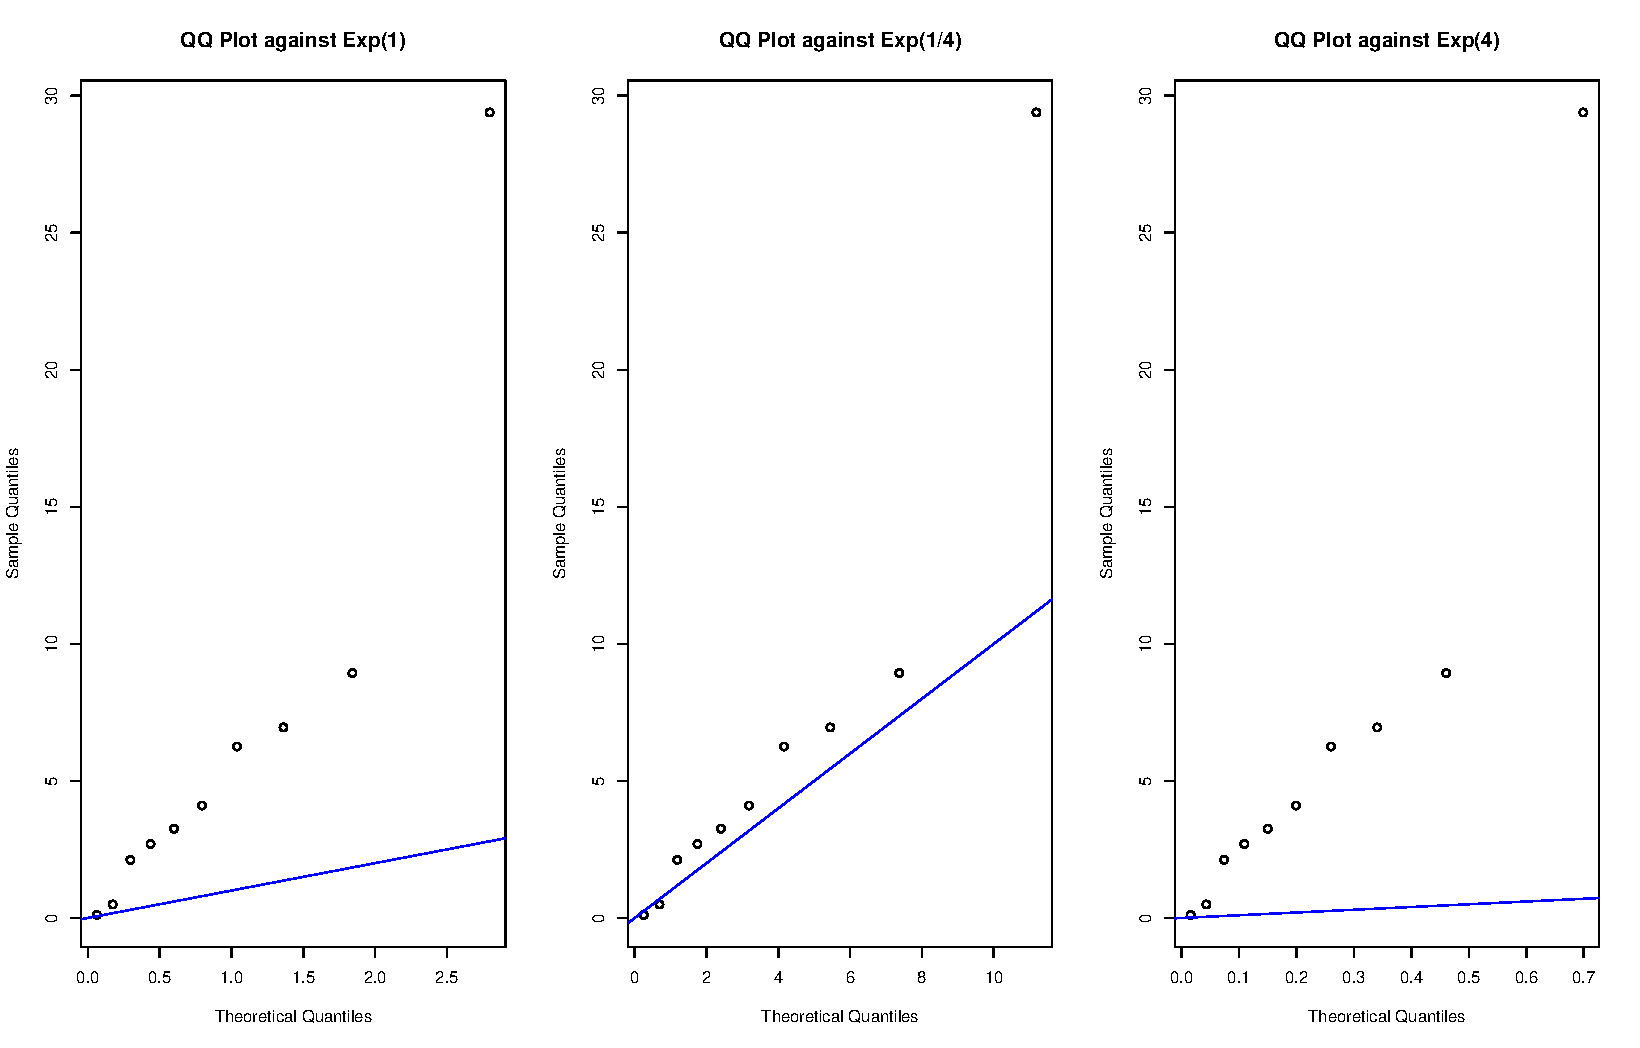
\includegraphics[width=\textwidth]{img/qqplot2-3.pdf}
The most compatible is the $Exp(1/4)$
\subsection*{2.3.2:}
\begin{center}
    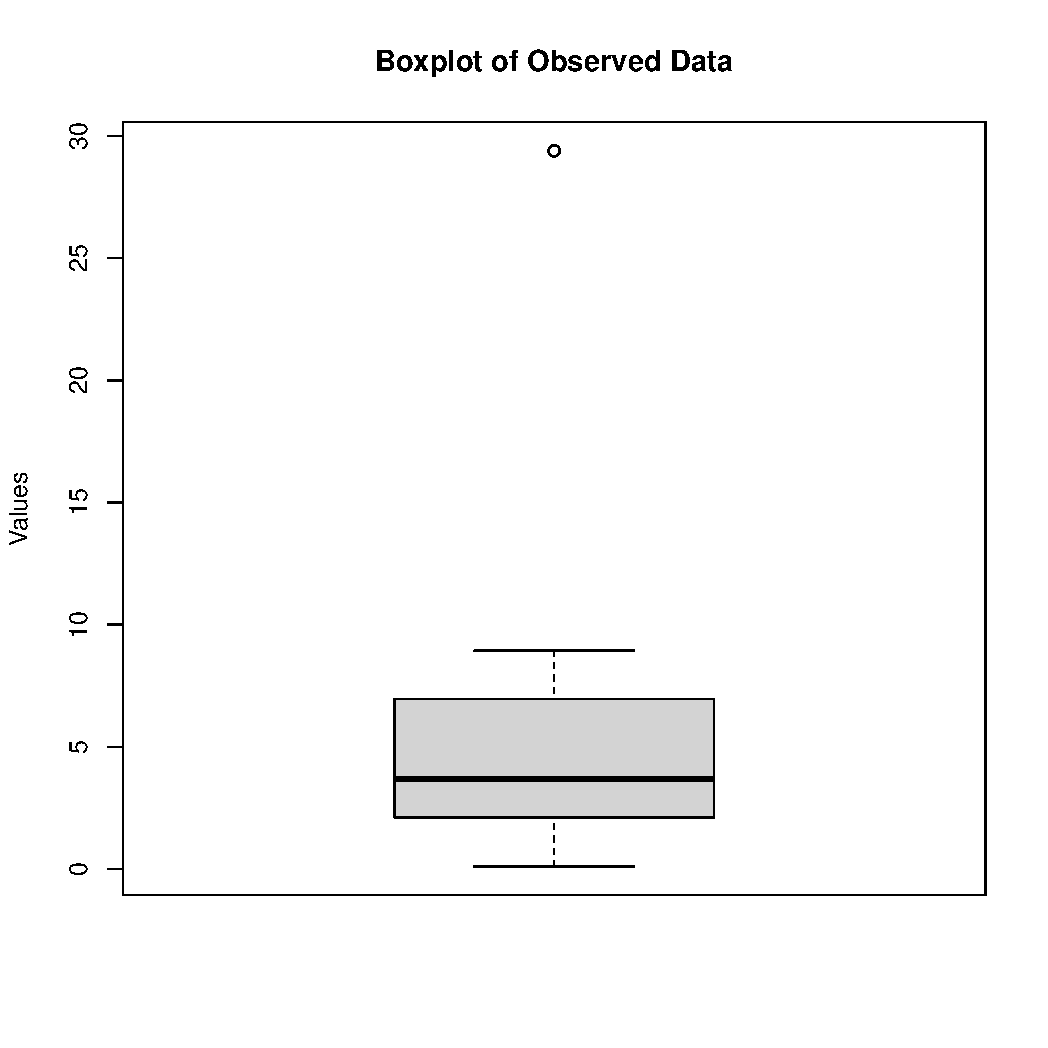
\includegraphics[width=.4\textwidth]{img/boxplot-2-3.pdf}
    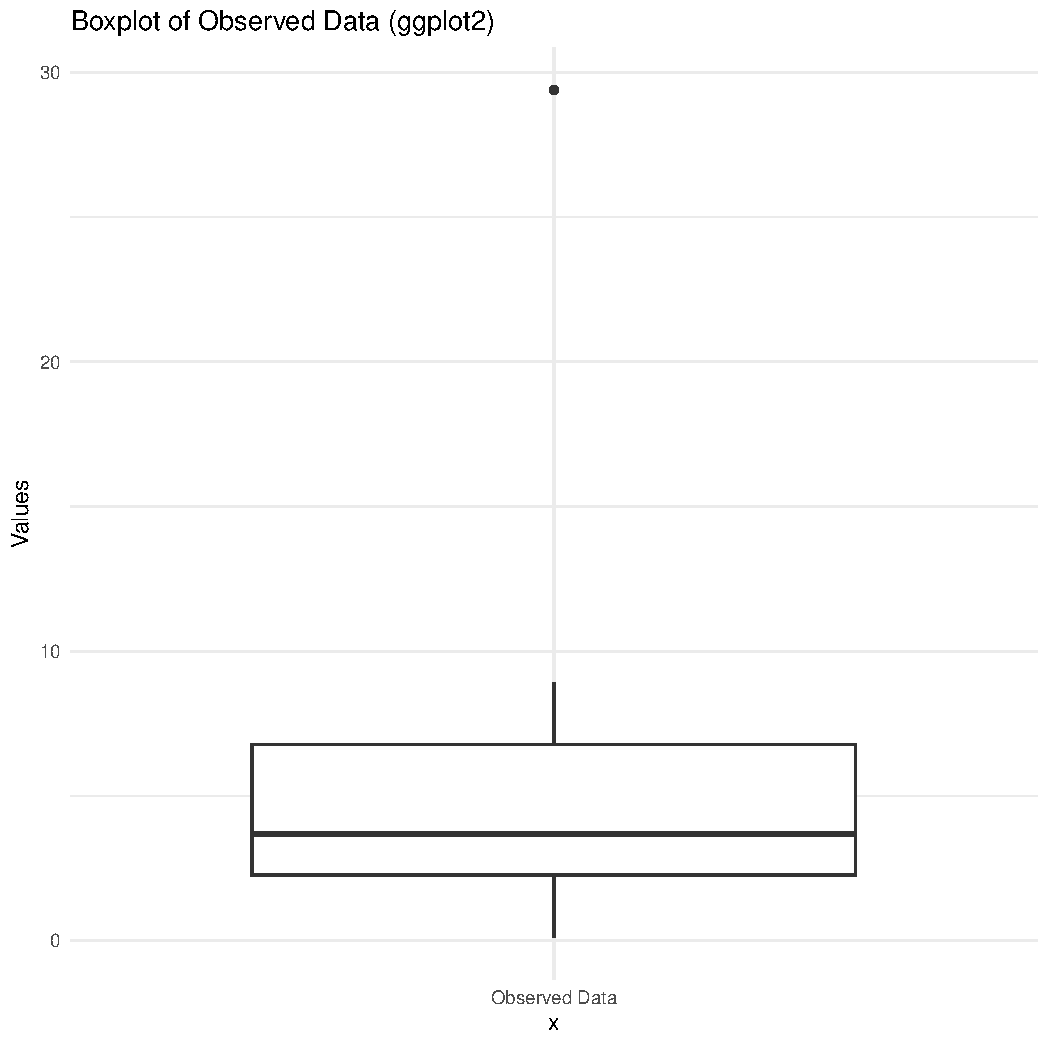
\includegraphics[width=.4\textwidth]{img/boxplot-2-3(1).pdf}
\end{center}
We can't spot any differences and the boxplot tells us that the distribution is "roughly" symmetric, since the whiskers are kinda of the same length.\\
The quantiles are roughly $Q_1=2,Q_2=4,Q_3=7$.\\
We can also see only one sample outside the boxplot, wich means that there is only a value $X_i$ s.t. $X_i\geq q_3+1.5\cdot iqr$.
\subsection*{2.3.3:}
$$\hat{F_n}(5.25)=\frac{1}{n}\sum_i\textbf{1}_{X_i}(x)=\frac{6}{10}=0.6$$
Running the following code in R, we get the same result:\\
\begin{verbatim}
data <- c(8.935, 0.492, 6.951, 4.102, 0.111, 2.699, 3.255, 6.254, 2.120, 29.389)
f <- ecdf(data)
f(5.25) # 0.6
\end{verbatim}

\end{document}